\chapter{实验}
本章将根据

% \section{公平性研究实验}
% 实验在SUMO(simulation of Urban MObility)\footnote{http://sumo.dlr.de/index.html}仿真平台上进行,利用该模拟器可以方便地实时获取车辆状态,并通过改变交通信号来控制交通运行。我们实现了一个四路交叉口作为我们的实验场景,
% 交叉口与四个150米长的路段相连,每条道路有三条引入车道和三条引出车道。

% 我们将N-S方向的道路设置为主干道,车辆到达量更多,将W-E方向的道路设置为次干道,车辆到达量较少。车辆到达服从泊松分布,这里我们设置N-S方向道路的交通流量比率为$\rho$,W-E方向道路的交通流量比率为$1-\rho$,$\rho$值越高,交通流量不平衡的状况越严重。
% 为了对我们的方法进行综合评价,我们在不同的$\rho$值下进行了实验。注意,为了简化环境,这里我们不考虑行人交通的影响。

% \subsection{评价指标}
% 我们使用以下指标来评估不同方法的效率和公平性表现:
% \begin{itemize}
%     \item 行驶时间:车辆行驶时间是指车辆进出路口的时间差。现有的大部分工作都集中在最小化所有车辆通过交叉路口的平均行驶时间。
%     \item 延误时间:车辆延误时间是车辆通过交叉路口的实际时间与预期时间(以最高限速通过交叉路口所需的时间)之间的差值。
%     \item 驾驶体验得分:此外,我们提出了一种新的评价指标,称为驾驶体验得分(Driving Experience Score,DES),来量化驾驶员的满意度,具体评分标准见下表:
%         \begin{table}[htb]
%             \caption{驾驶体验得分标准}
%             \begin{tabular}{cc}
%             \toprule
%             延误时间(s) & DES \\
%             \midrule
%             $d \leq 40$ & 5\\
%             $40 < d \leq 80$ & 4 \\
%             $80 < d \leq 120$ & 3 \\
%             $120 < d \leq 160$ & 2 \\
%             $d > 160$ & 1 \\ 
%             \bottomrule
%             \end{tabular}
%         \end{table}
%         事实上,可能有更多的因素需要考虑(如燃油消耗),但是这里的目的是为了缓解车辆的过度延误情况,因此我们这里用延误时间作为评价标准。
% \end{itemize}
% \subsection{比较方法}
% \begin{itemize}
%     \item FT(Fixed-Time Control\cite{miller1963settings}):这种方法以预先设定的方式循环改变信号。
%     \item SOTL(Self-Organizing Traffic Light Control\cite{cools2013self}):这是一种根据预先设定的阈值来改变信号的自适应方法。如果等待的车辆数量超过了这个阈值,则切换到下一个信号相位。
%     \item LIT\cite{zheng2019diagnosing}:这是一种基于学习的方法,比大多数现有的致力于提高通行效率的方法效果更好。
%     \item FIT(\textbf{F}airness-aware \textbf{I}ntelligent \textbf{T}raffic Light Control):我们的方法。
% \end{itemize}
% \subsection{性能评价}
% 首先,我们通过实验评估了不同方法的通信效率的表现,为了得到一个综合的结果,我们在不同的$\rho$值下进行了实验,实验结果如\autoref{fig:efficiency}所示。
% 可以观察到,我们的方法(FIT)的车辆通过路口的平均行驶时间远低于传统方法(行驶时间越短意味着效率越高),并且仅略低于只注重效率的LIT方法。
% \begin{figure}[htb]
%     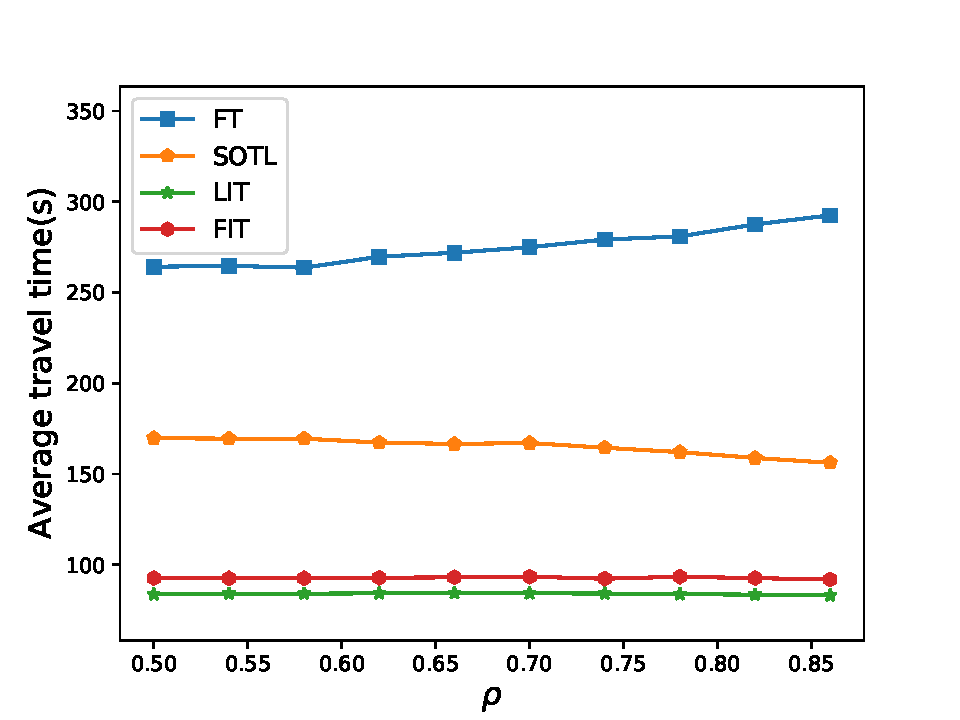
\includegraphics[width=10cm]{fig/efficiency.pdf}
%     \caption{效率}
%     \label{fig:efficiency}
% \end{figure}

% 其次,由于我们的主要研究目标是公平性,我们首先分析了在使用不同方法下每条车道的延误情况。这里我们用Jain Fairness Index(JFI)来量化公平性指标,JFI的计算方式如下:
% \begin{align}
%     \mathcal{J}=\frac{\left(\sum_{i=1}^{M} \bar{D}_{i}\right)^{2}}{M \sum_{i=1}^{M} \bar{D}_{i}^{2}},
% \end{align}
% 其中$\bar{D}_{i}$是车道$i$的平均延误时间。当每个车道具有相同的平均延误时间时,JFI的值达到最大值,即1。\autoref{fig:fairness}展示了四种方法在不同$\rho$值下的平均延迟的JFI表现。从中我们可以看出FT和LIT的JFI值随着交通不平衡情况的加剧(即$\rho$值越大)而减小,而FIT任然能偶保持较高的值,并且高于同样能够保持稳定JFI值的SOTL方法。
% \begin{figure}[htb]
%     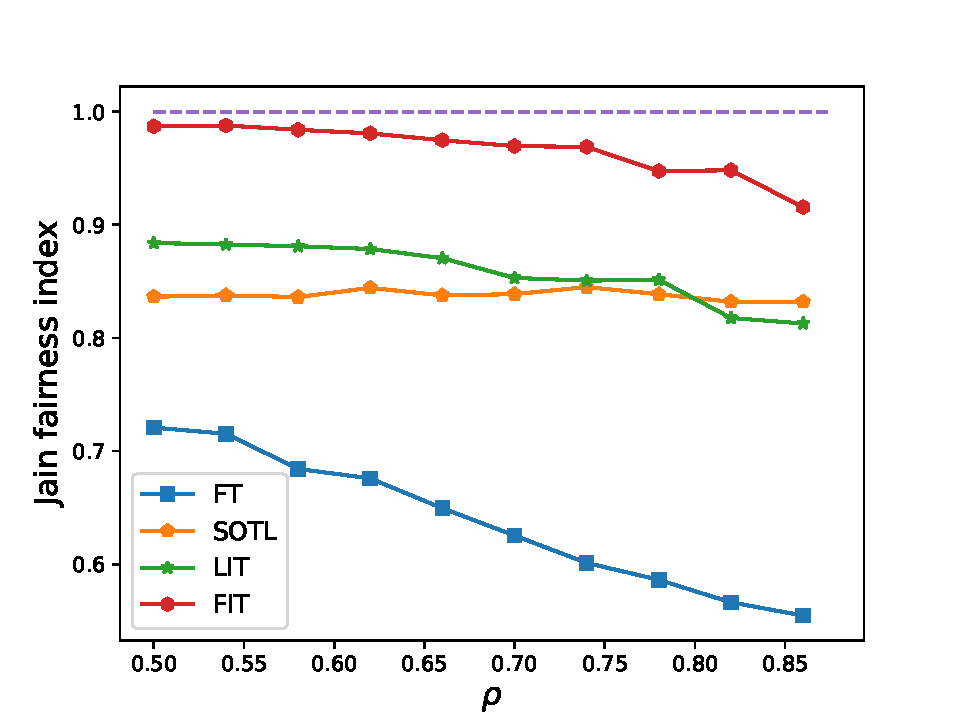
\includegraphics[width=10cm]{fig/fairness.pdf}
%     \caption{公平}
%     \label{fig:fairness}
% \end{figure}

% 然后,我们更加详细地研究了不同方法的延误情况。下面我们具体分析在主干道和支干道上四种方法在不同的$\rho$值情况下车辆延误时间分布情况。
% \begin{figure}[htb]
%     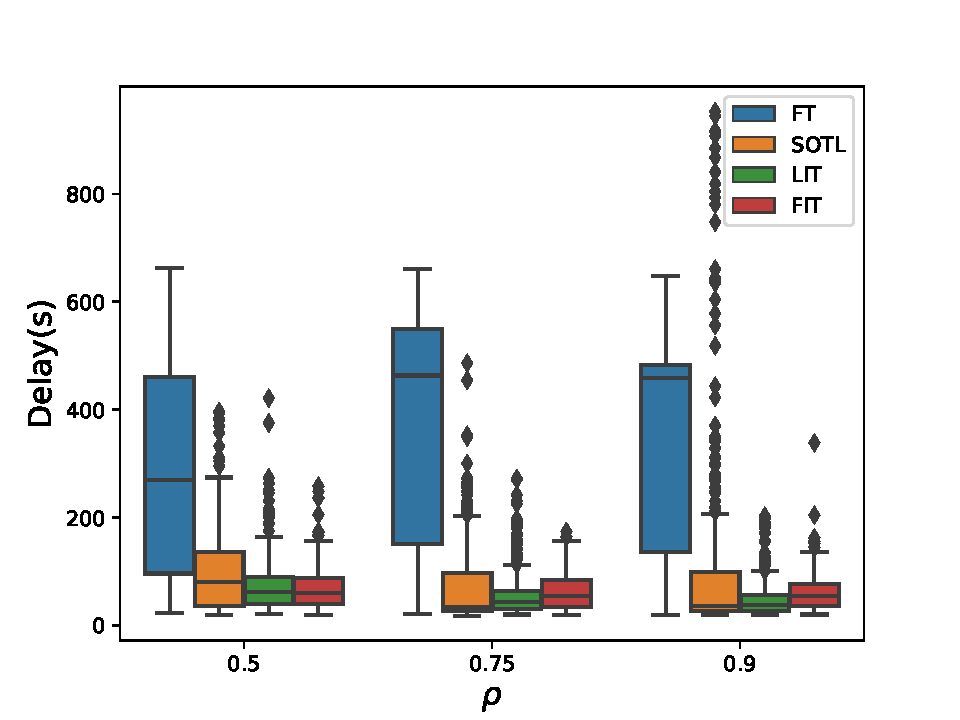
\includegraphics[width=10cm]{fig/major_delay.pdf}
%     \caption{主干道(N-S方向)的车辆延误时间分布}
%     \label{fig:major_delay}
% \end{figure}
% 从\autoref{fig:major_delay}中我们可以看出,在主干道上,基于学习的方法(LIT和FIT)比传统方法(FT和SOTL)具有更低的延误时间,虽然SOTL方法整体上延迟也比较低,但是会有很多极端值,最高的延误时间甚至超过800$s$。

% 从\autoref{fig:minor_delay}中我们可以看出,在支干道上,随着$\rho$值的增加(即交通不平衡情况的加重),原先在主干道上表现优异的LIT方法性能开始恶化(),但是FIT依然能够保持一个相对低的延迟。

% \begin{figure}[htb]
%     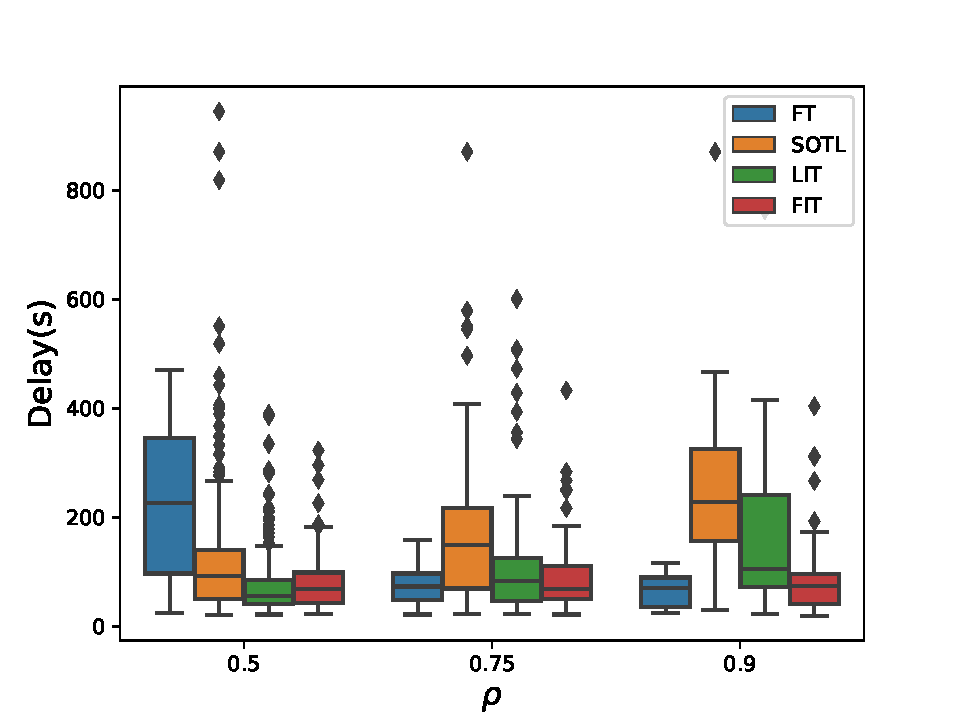
\includegraphics[width=10cm]{fig/minor_delay.pdf}
%     \caption{支干道(N-S方向)的车辆延误时间分布}
%     \label{fig:minor_delay}
% \end{figure}

% 最后我们研究了不同方法的驾驶体验得分情况,\autoref{fig:des}展示了在$\rho=0.75$的情况下不同方法的驾驶体验得分分布情况。从中我们可以看出,FT方法超过半数的驾驶体验的分都是1分,由此可以看出该方法的不灵活。对于SOTL方法而言,虽然他的5分的比例最高,但是其得分分布的方差也是最高的。FIT的得分分布与LIT相似,但FIT的方差低于LIT,在以牺牲少量效率为代价的前提下。
% % \begin{figure}[t]
% %     \subfloat[FT]{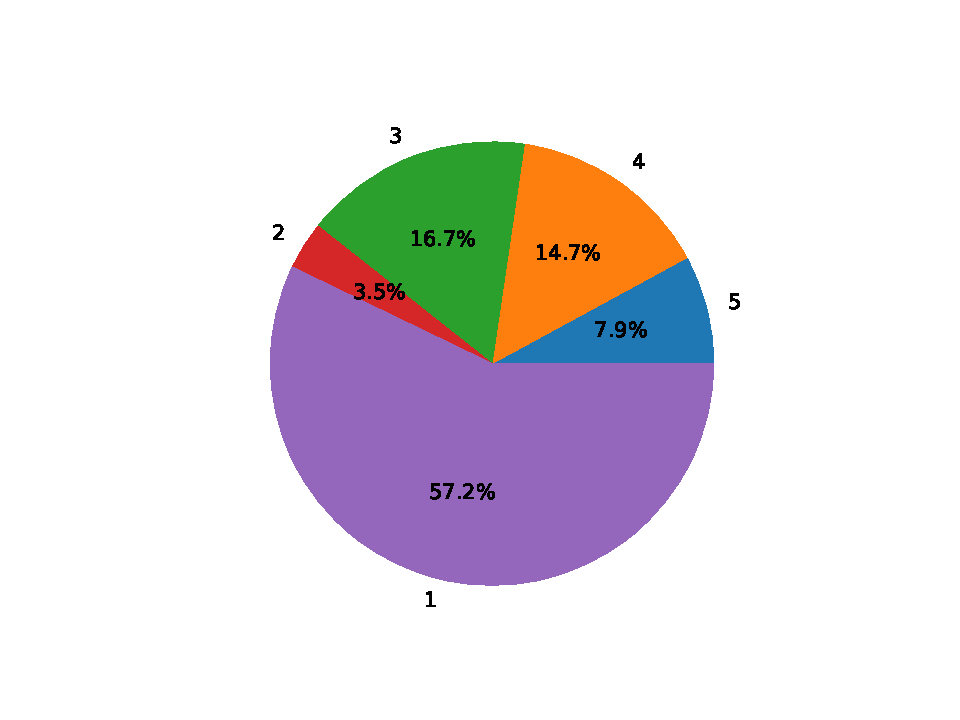
\includegraphics[width=.4\textwidth]{fig/score_FT.pdf}}\quad
% %     \subfloat[SOTL]{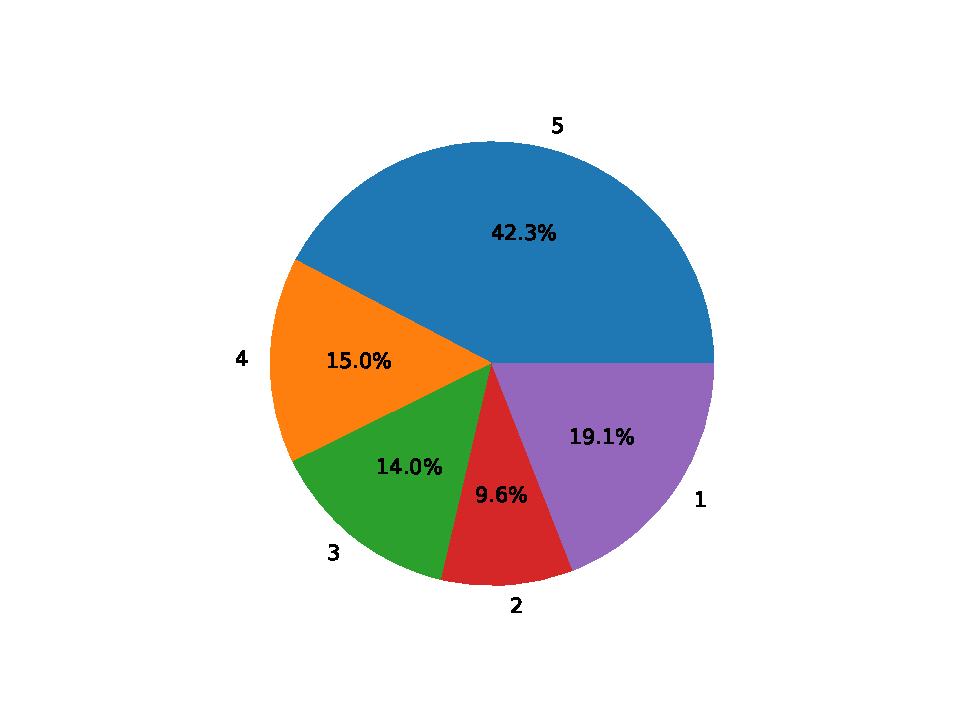
\includegraphics[width=.4\textwidth]{fig/score_SOTL.pdf}}\\
% %     \subfloat[LIT]{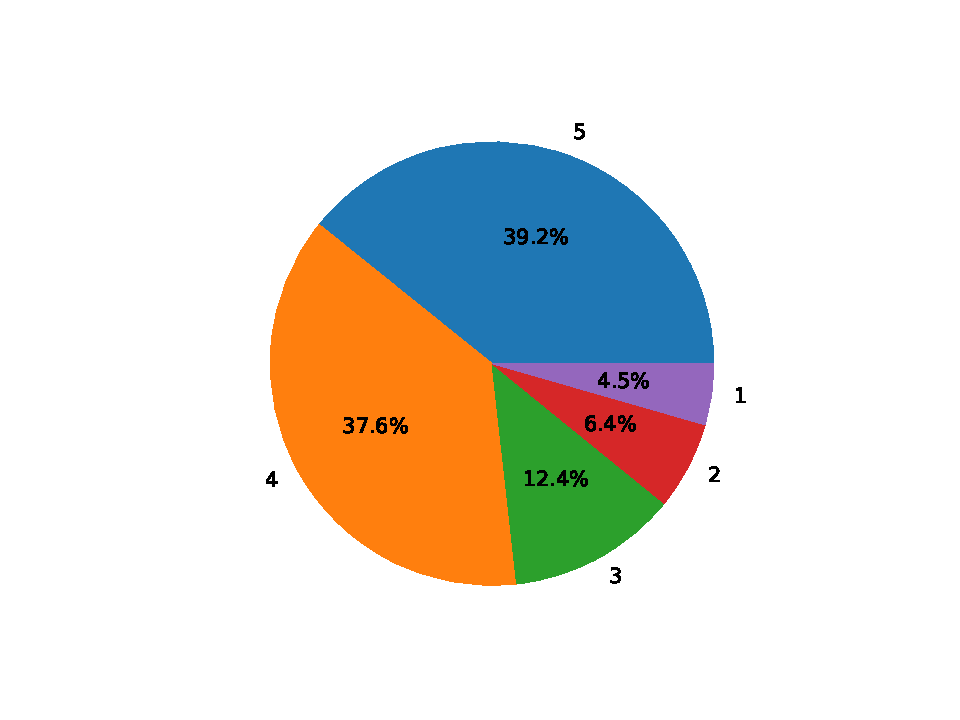
\includegraphics[width=.4\textwidth]{fig/score_LIT.pdf}}\quad
% %     \subfloat[FIT]{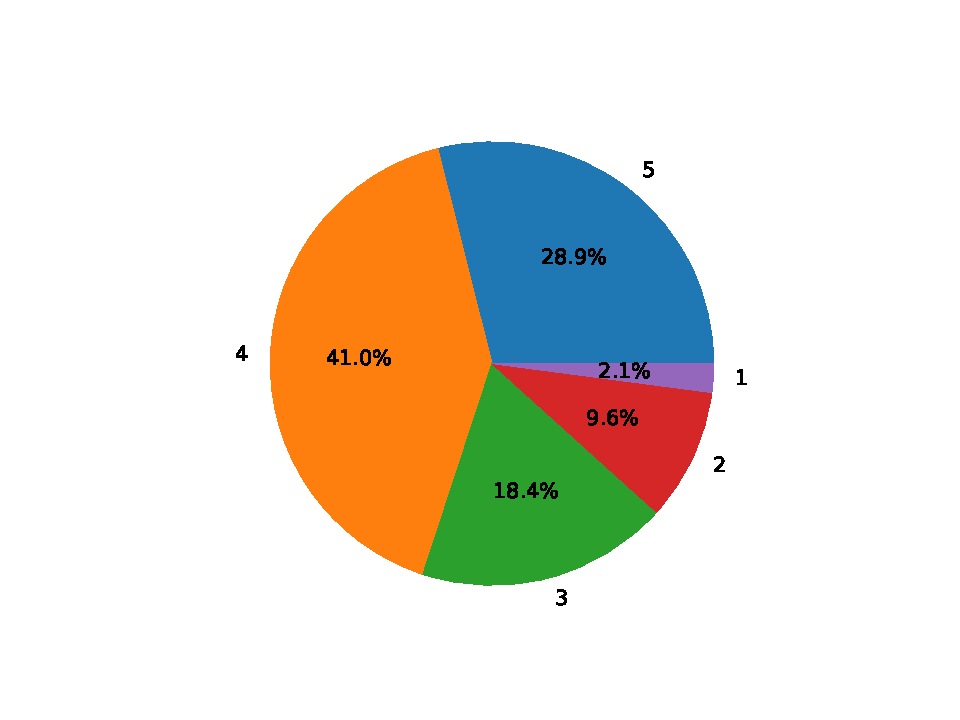
\includegraphics[width=.4\textwidth]{fig/score_FIT.pdf}}
% %     \caption{驾驶体验得分统计}
% %     \label{fig:des}
% %   \end{figure}

% \begin{figure}[t]
%     \centering
%     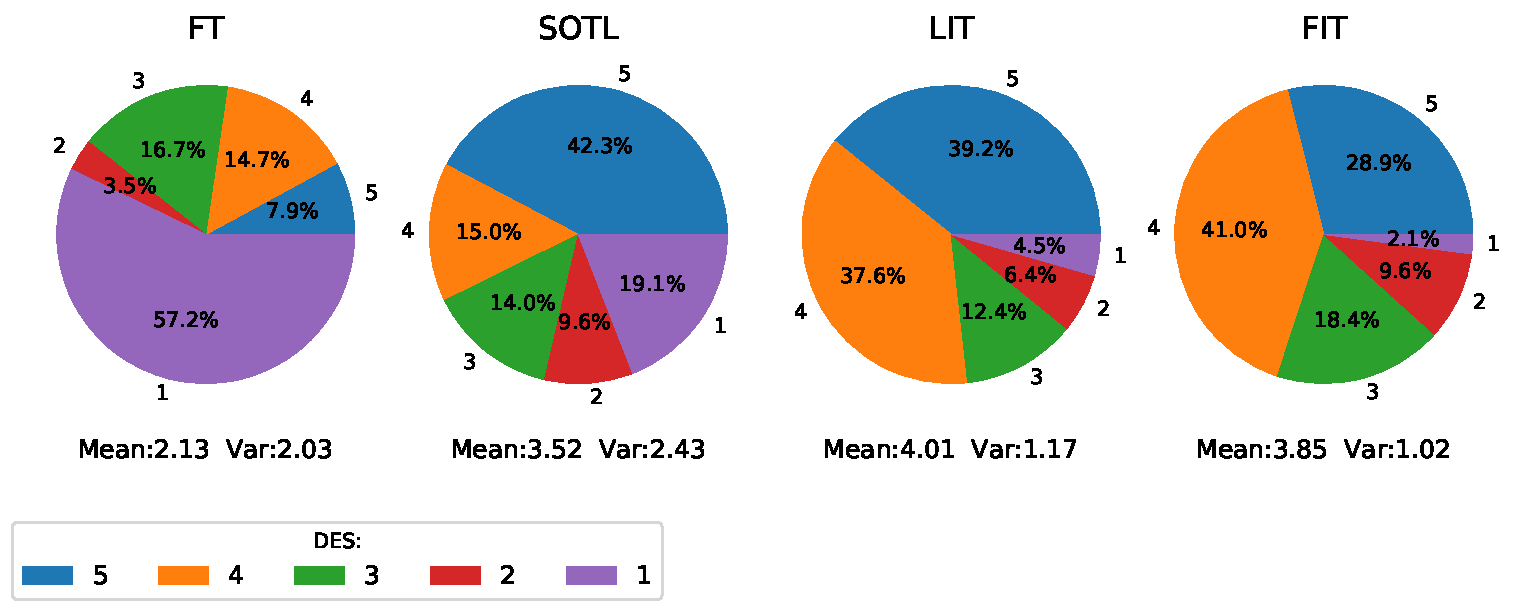
\includegraphics[width=0.9\textwidth]{fig/des.pdf}
%     \caption{驾驶体验得分统计}
%     \label{fig:des}
% \end{figure}

